\documentclass[a4paper]{article}

\usepackage[T1]{fontenc}
\usepackage[utf8]{inputenc}
\usepackage{mlmodern}

%\usepackage{ngerman}	% Sprachanpassung Deutsch

\usepackage{graphicx}
\usepackage{geometry}
\geometry{a4paper, top=15mm}

\usepackage{subcaption}
\usepackage[shortlabels]{enumitem}
\usepackage{amssymb}
\usepackage{amsthm}
\usepackage{amsmath}
\usepackage{mathtools}
\usepackage{braket}
\usepackage{bbm}
\usepackage{graphicx}
\usepackage{float}
\usepackage{yhmath}
\usepackage{tikz}
\usepackage{scratch}
\usetikzlibrary{patterns,decorations.pathmorphing,positioning}
\usetikzlibrary{calc,decorations.markings}

\usepackage[backend=biber, sorting=none]{biblatex}
\addbibresource{cite.bib}

\usepackage[framemethod=TikZ]{mdframed}

\tikzstyle{titlered} =
    [draw=black, thick, fill=white,%
        text=black, rectangle,
        right, minimum height=.7cm]


\usepackage[colorlinks=true,naturalnames=true,plainpages=false,pdfpagelabels=true]{hyperref}
\usepackage[parfill]{parskip}
\usepackage{lipsum}

\usepackage{tcolorbox}
\tcbuselibrary{skins,breakable}

\pagestyle{myheadings}

\colorlet{colexam}{black}
\newcounter{definition}
\newtcolorbox[use counter=definition]{mydef}[1]{
    empty,
    title={\textbf{Definition~\thetcbcounter}~~(\textit{#1})},
    attach boxed title to top left,
    fontupper=\sl,
    boxed title style={
        empty,
        size=minimal,
        bottomrule=1pt,
        top=1pt,
        left skip=0cm,
        overlay=
            {\draw[colexam,line width=1pt]([yshift=-0.4cm]frame.north
        west)--([yshift=-0.4cm]frame.north east);}},
            coltitle=colexam,
            fonttitle=\normalfont,
            before=\par\medskip\noindent,
            parbox=false,
            boxsep=-1pt,
            left=0.75cm,
            right=3mm,
            top=4pt,
            breakable,
            pad at break*=0mm,
            vfill before first,
            overlay unbroken={
                \draw[colexam,line width=1pt]
                ([xshift=0.6cm, yshift=-0.5pt]frame.south
                west)--([xshift=0.6cm,yshift=-1pt]frame.north west)
                --([xshift=0.6cm]frame.south west)--([xshift=-13cm]frame.south east); },
            overlay first={
                \draw[colexam,line width=1pt]
                ([xshift=0.6cm, yshift=-0.5pt]frame.south
                west)--([xshift=0.6cm,yshift=-1pt]frame.north west)
                --([xshift=0.6cm]frame.south west); },
            overlay last={
                \draw[colexam,line width=1pt]
                ([xshift=0.6cm, yshift=-0.5pt]frame.south
                west)--([xshift=0.6cm,yshift=-1pt]frame.north west)
                --([xshift=0.6cm]frame.south west)--([xshift=-13cm]frame.south east); }
}
\newcounter{theorem}
\newtcolorbox[use counter=theorem]{theorem}{
    empty,
    title={Theorem ~\thetcbcounter},
    attach boxed title to top left,
    fontupper=\sl,
    boxed title style={
        empty,
        size=minimal,
        bottomrule=1pt,
        top=1pt,
        left skip=0cm,
        overlay=
            {\draw[colexam,line width=1pt]([yshift=-0.4cm]frame.north
        west)--([yshift=-0.4cm]frame.north east);}},
            coltitle=colexam,
            fonttitle=\bfseries,
            before=\par\medskip\noindent,
            parbox=false,
            boxsep=-1pt,
            left=0.75cm,
            right=3mm,
            top=4pt,
            breakable,
            pad at break*=0mm,
            vfill before first,
            overlay unbroken={
                \draw[colexam,line width=1pt]
                ([xshift=0.6cm, yshift=-0.5pt]frame.south
                west)--([xshift=0.6cm,yshift=-1pt]frame.north west)
                --([xshift=0.6cm]frame.south west)--([xshift=-13cm]frame.south east); },
            overlay first={
                \draw[colexam,line width=1pt]
                ([xshift=0.6cm, yshift=-0.5pt]frame.south
                west)--([xshift=0.6cm,yshift=-1pt]frame.north west)
                --([xshift=0.6cm]frame.south west); },
            overlay last={
                \draw[colexam,line width=1pt]
                ([xshift=0.6cm, yshift=-0.5pt]frame.south
                west)--([xshift=0.6cm,yshift=-1pt]frame.north west)
                --([xshift=0.6cm]frame.south west)--([xshift=-13cm]frame.south east); }
}
\newcounter{lemma}
\newtcolorbox[use counter=lemma]{lemma}{
    empty,
    title={Lemma~\thetcbcounter},
    attach boxed title to top left,
    fontupper=\sl,
    boxed title style={
        empty,
        size=minimal,
        bottomrule=1pt,
        top=1pt,
        left skip=0cm,
        overlay=
            {\draw[colexam,line width=1pt]([yshift=-0.4cm]frame.north
        west)--([yshift=-0.4cm]frame.north east);}},
            coltitle=colexam,
            fonttitle=\bfseries,
            before=\par\medskip\noindent,
            parbox=false,
            boxsep=-1pt,
            left=0.75cm,
            right=3mm,
            top=4pt,
            breakable,
            pad at break*=0mm,
            vfill before first,
            overlay unbroken={
                \draw[colexam,line width=1pt]
                ([xshift=0.6cm, yshift=-0.5pt]frame.south
                west)--([xshift=0.6cm,yshift=-1pt]frame.north west)
                --([xshift=0.6cm]frame.south west)--([xshift=-13cm]frame.south east); },
            overlay first={
                \draw[colexam,line width=1pt]
                ([xshift=0.6cm, yshift=-0.5pt]frame.south
                west)--([xshift=0.6cm,yshift=-1pt]frame.north west)
                --([xshift=0.6cm]frame.south west); },
            overlay last={
                \draw[colexam,line width=1pt]
                ([xshift=0.6cm, yshift=-0.5pt]frame.south
                west)--([xshift=0.6cm,yshift=-1pt]frame.north west)
                --([xshift=0.6cm]frame.south west)--([xshift=-13cm]frame.south east); }
}

\newcommand{\eps}{\varepsilon}
\usepackage[OT2,T1]{fontenc}
\DeclareSymbolFont{cyrletters}{OT2}{wncyr}{m}{n}
\DeclareMathSymbol{\Sha}{\mathalpha}{cyrletters}{"58}

\markright{Popović\hfill Seminar\hfill}


\title{University of Vienna\\
\vspace{1cm}Seminar:\\Joint RICAM Seminar\\
\vspace{0.5cm}
Summary of talk by Otmar Scherzer
}
\author{Milutin Popovic}


\begin{document}
\maketitle
\tableofcontents

\section{Sheet 8}
\subsection{Finite Discrete Fourier Transform (FDFT)}
Consider the vector $\begin{pmatrix}a & b & c & d\end{pmatrix}^T \in
\mathbb{C}^4$ with a FDFT $\begin{pmatrix}A & B & C & D\end{pmatrix}^T$. We
can show that the vector
\begin{align}
    \begin{pmatrix}a & 0 & b & 0 & c & 0 & d & 0\end{pmatrix}^T,
\end{align}
has the FDFT of
\begin{align}
    \frac{1}{2}\begin{pmatrix}A & 0 & B & 0 & C & 0 & D & 0\end{pmatrix}^T.
\end{align}
For the $N=4$, $n\in\{0,\dots,3\}$ the coefficients $a, b, c, d$ are denoted in
$f[n]$. The FDFT is
\begin{align}
    \hat{f}[k] &= \frac{1}{4} * \sum_{n=0}^3 f[n] e^{-2\pi i \frac{n}{4}k} \\
               &=\frac{1}{4}\left(
                   a + be^{-\pi i \frac{k}{2}}
                   + ce^{-\pi i k}+ de^{-\frac{3\pi i k}{2}}
               \right) = \\
    (&=\begin{pmatrix}A & B & C & D\end{pmatrix}^T)
\end{align}
for $k \in \{0,\dots, 3\}$ accordingly. For the $N=8$, $\mathbb{C}^8$ case
 we have $f_2[n]$ for $n \in \{0,\dots 7\}$,
 \begin{align}
    \hat{f}_2[k] &= \frac{1}{8} * \sum_{n=0}^7 f_2[n] e^{-2\pi i \frac{n}{8}k} \\
               &=\frac{1}{2}\frac{1}{4}\left(
                   a + be^{-\pi i \frac{k}{2}}
                   + ce^{-\pi i k}+ de^{-\frac{3\pi i k}{2}}
               \right) = \\
    (&=\frac{1}{2}\begin{pmatrix}A & B & C & D & A & B & C & D\end{pmatrix}^T)
 \end{align}
for $k \in \{0,\dots, 7\}$ accordingly. We may generalize now for
$\mathbb{C}^{4N}$, and the sequence for $a, b, c, d, 0$ represented by the
function $g[n]$ for $n \in \{0,\dots, 4N-1\}$,
\begin{align}
    g[n] =\begin{cases}
        f[n] \qquad n\in \{0, N, 2N, 3N\}\\
        0 \qquad \text{else}
        \end{cases}.
\end{align}
Now we can compute the FDFT for $k \in \{0,\dots, 4N-1\}$
\begin{align}
    \hat{g}[k] &= \frac{1}{4N}\sum_{n=0}^{4N-1} g[n]e^{-2\pi i
    \frac{n}{4N}k}\\
         &=\frac{4}{N}\sum_{n=0}{3}f[n]e^{-2\pi i \frac{n}{4}k}\\
         &=\frac{1}{N}\left(\frac{1}{4}\sum_{n=0}^3 f[n] e^{-2\pi i
         \frac{n}{4}k} \right) \\
         &= \frac{1}{N} \underbrace{\begin{pmatrix}A & B & C & D & \dots &
             \dots & A & B & C & D\end{pmatrix}^T)}_{\text{$4N$ entries, $N$
         sequences}}.
\end{align}
\subsection{More FDFT}
Consider the discrete complex exponential with frequency of $1Hz$ in
$\mathbb{C}^8$, for $n \in \{0, \dots , 7\}$,
\begin{align}
    \exp[n] = e^{2\pi i n/8}.
\end{align}
The FDFT for $k \in \{0, \dots, 7\}$ is
\begin{align}
    \hat{\exp}[k] &= \frac{1}{8}\sum_{n=0}^7 e^{2\pi i \frac{n}{8}}e^{-2\pi i
    n \frac{k}{8}} \\
                  &= \frac{1}{8} \sum_{n=0}^7e^{-2\pi i (k-1)\frac{n}{8}}\\
                  &=
                  \begin{cases}
                      1\quad k=1\\
                      0 \qquad k\neq 1
                   \end{cases}.
\end{align}
\begin{figure}[H]
    \centering
    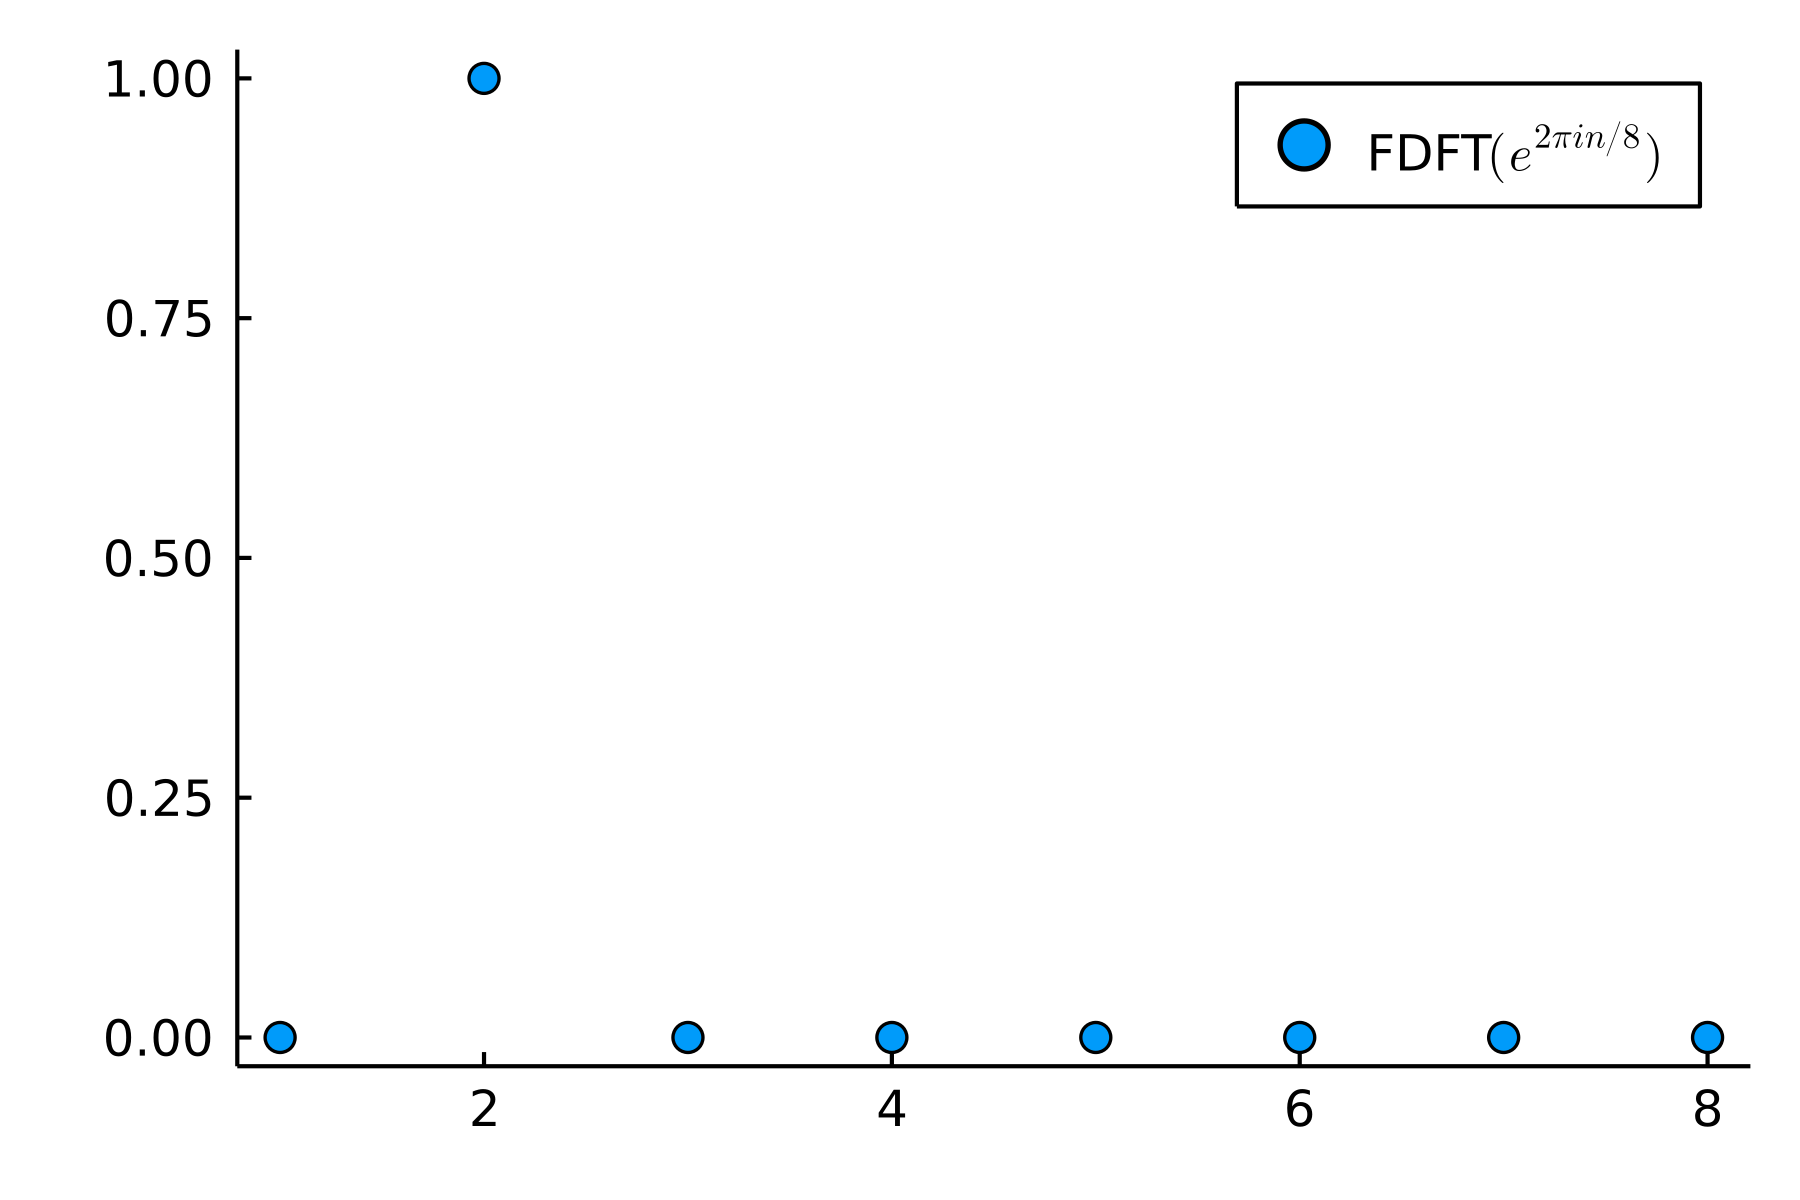
\includegraphics[width=0.49\textwidth]{./figures/fdft.png}
    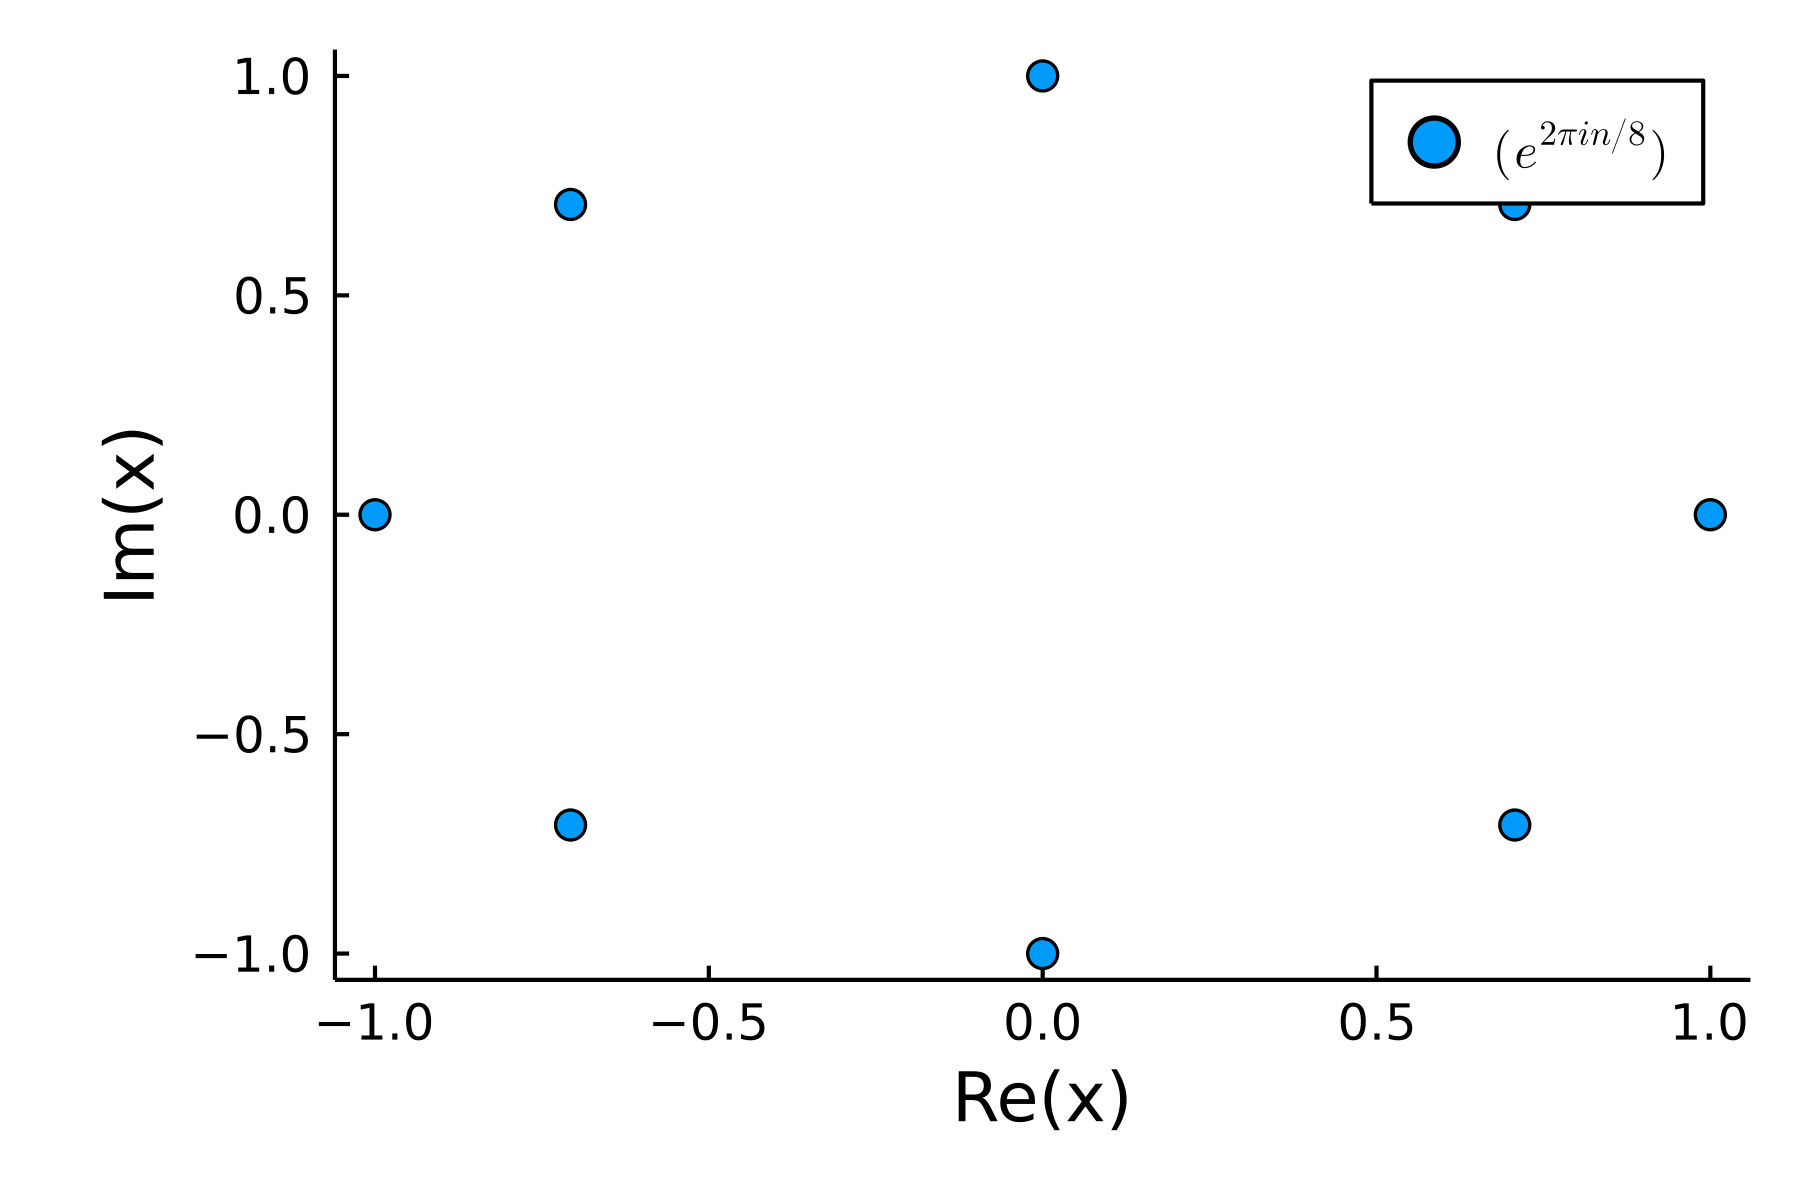
\includegraphics[width=0.49\textwidth]{./figures/normal.png}
    \caption{Test in Julia}
\end{figure}
\subsection{Sampling Sinusoids}
Consider the following continuous signal
\begin{align}
    f(t) = sin(20\pi t) + sin(40\pi t)
\end{align}
with frequencies $\omega = 2\pi \nu$, $\nu_1 = 10\ \text{Hz}$ and $\nu_2 = 20\
\text{Hz}$. Sketching its Fourier transform would be something like this
\begin{figure}[H]
    \centering
\begin{tikzpicture}[
    axisline/.style={very thick, -stealth},
    xscale = 1.5,
    yscale = 1.5
    ]
    \draw[axisline] (-3,0)--(3,0) node[right]{$\nu$};
    \draw[axisline] (0,-1.5)--(0,1.5) node[above]{$\hat{f}$};
    \draw[->] (-1,0) -- (-1, -1) node[below] {$-\delta(\nu - 10)$};
    \draw[->] (-2,0) -- (-2, 1) node[above] {$\delta(\nu - 20)$};
    \draw[->] (1,0) -- (1, 1) node[above] {$\delta(\nu - 10)$};
    \draw[->] (2,0) -- (2, 1) node[above] {$\delta(\nu - 20)$};
\end{tikzpicture}
\end{figure}
The Nyquist frequency for sampling would be
\begin{align}
    \nu_{\text{Nyquist}} = 2\nu_\text{max} = 2\nu_2 = 40\ \text{Hz},
\end{align}
If we choose $50\ \text{Hz}$ for sampling we would get aliasing with the
following frequencies
\begin{align}
    n \cdot 50\ \text{Hz} - 20\ \text{Hz} = 30\ \text{Hz},80\ \text{Hz}, 130\
    \text{Hz}, \dots
\end{align}
\subsection{Short-Time Fourier Transform (STFT)}
The Definition of the STFT is
\begin{align}
    \text{STFT}\{f\} &= S_\varphi f(\tau, \omega) = \int_\mathbb{R} f(t)
    \overline{\text{M}_\omega \text{T}_\tau \varphi}dt \\
                 &=\int_\mathbb{R} f(t)
    \bar{\varphi}(t - \tau)e^{-2\pi i \omega t}\ dt \\
\end{align}
Then we have the following identity
\begin{align}
    S_\varphi(\text{T}_u\text{M}_\eta f)(x,\omega)
    &= \int_\mathbb{R}
     \left(\text{T}_u \text{M}_\eta f(t)\right) \bar{\varphi}(t-x) e^{-2\pi i
         \omega t}\ dt\\
    &= \int_\mathbb{R} e^{2\pi i \eta(t-u)}f(t-u) e^{-2\pi i \omega
    t}\bar{\varphi}(t-x)\ dt \qquad \text{(sub: $s = t-u$)}\\
    &= \int_\mathbb{R} f(s)\bar{\varphi}(s-(x-u))e^{2\pi i \eta s}e^{-2\pi i
    \omega s} e^{-2\pi i \omega u}\ ds \\
    &=e^{-2\pi i \omega u}\int_\mathbb{R} f(s) \bar{\varphi}(s-(x-u))e^{-2\pi i
    (\omega - \eta)s}\ ds\\
    &=e^{-2\pi i \omega u}\int_\mathbb{R}
    f(s)\overline{ \text{M}_{(\omega-\eta)} \text{T}_{(x-u)}\varphi(s)}\ ds\\
    &=e^{-2\pi i \omega u} S_\varphi f\left(x-u,\ \omega -\eta\right).
\end{align}
The second identity we can show
\begin{align}
    S_\varphi f(x, \omega)
    &= \langle f, \overline{\text{M}_\omega \text{T}_x \varphi}\rangle \\
    &= \langle\mathcal{F} f, \mathcal{F} \overline{\text{M}_\omega \text{T}_x \varphi}\rangle \\
    &= \int_\xi \hat{f}(\xi)\int_t \overline{\text{M}_\omega \text{T}_x
    \varphi}(t) e^{-2\pi i \xi t}\ dt\ d\xi \\
    &= \int_\xi \hat{f}(\xi)\int_t \hat{\bar{\varphi}}(t-x) e^{2\pi i \omega
    t} e^{-2\pi i \xi t}\ dt\ d\xi \\
    &= \int_\xi \hat{f}(\xi)\int_t \hat{\bar{\varphi}}(t-x)e^{-2\pi i (\xi
    -\omega)t}\ dt\ d\xi \qquad \text{sub $u=t-x$}\\
    &= \int_\xi \hat{f}(\xi)\int_t \hat{\bar{\varphi}}(u)e^{-2\pi i (\xi
    -\omega)u}e^{-2\pi i (\xi -\omega)x} \ dt\ d\xi\\
    &= \int_\xi \hat{f}(\xi)e^{-2\pi i (\xi -\omega)x}\int_t
    \hat{\varphi}(u)e^{-2\pi i (\xi -\omega)u} \ dt\ d\xi\\ &= e^{2\pi i
    \omega x}\int_\xi \hat{f}(\xi) \hat{\bar{\varphi}}(\xi - \omega) e^{-2\pi
    i \xi x}d\xi\\
    &= e^{2\pi i \omega x} S_{\hat{\varphi}} \hat{f}(\omega, -x).
\end{align}
% printbibliography
\end{document}
